\section{Interface Specification}
\label{sec:InterfaceSpecification}

Reusable components and patterns used to create custom components offer their functionality via public-facing interfaces. A detailed specification of these interfaces is required to enable an integration of all subsystems. Additionally, each subsystem defines artifacts that they produce for and consume from other components. The following section demonstrates the internal structure of custom components while for reused third-party subsystems their integration and emitted artifacts are illustrated.

\begin{figure}[!h]
	\centering{
		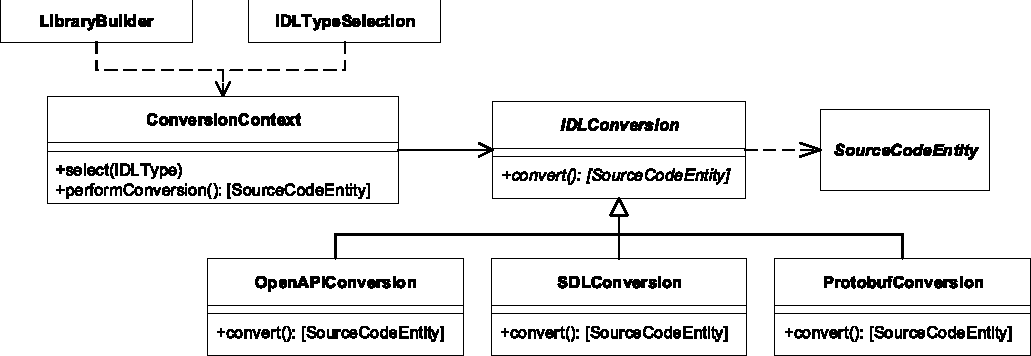
\includegraphics[width=150mm]{images/cd_idl_import.pdf}
		\caption{Class diagram of IDL importer subsystem}
		\label{fig:cdIDLImport}
	}
\end{figure}

Importing an \ac{IDL} for a specific type of Web API needs to flexibly switch between different implementations for various kinds of \acp{IDL}. Therefore, the strategy pattern is used to abstract the internal implementation from the consuming client code. The \texttt{LibraryBuilder} is the client that uses the \texttt{performConversion} method. Depending on the type of IDL which was set by the \texttt{IDL\-Type\-Selec\-tion} for the \texttt{ConversionContext}, the appropriate implementation of \texttt{IDL\-Con\-ver\-sion} performs the conversion and returns a list of \texttt{SourceCodeEntity} objects. 

\begin{figure}[!h]
	\centering{
		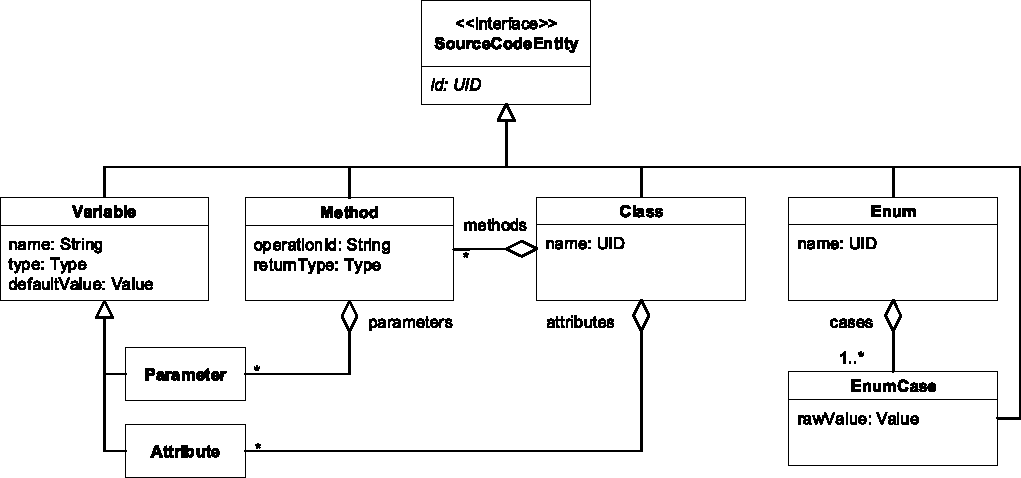
\includegraphics[width=150mm]{images/cd_sourceentity.pdf}
		\caption{Class diagram of source code entity artifact}
		\label{fig:cdSourceCodeEntity}
	}
\end{figure}

\texttt{SourceCodeEntity} objects are used by multiple components. They represent the basic syntactical elements that are common in all modern programming languages. Figure \ref{fig:cdSourceCodeEntity} shows their composition and their most important attributes and relations. \texttt{Class}, \texttt{Method} and \texttt{Enum} entities represent structual elements in which other elements can be nested. A \texttt{Class} element contains \texttt{Attributes} and \texttt{Methods}, whereas \texttt{Enums} specify at least one \texttt{EnumCase}. Each \texttt{Source\-Code\-Entity} can be identified by a \ac{UID}. For \texttt{Class} and \texttt{Enum} elements, their name itself is unique, while for \texttt{Variables}, \texttt{Methods} and \texttt{EnumCases} their context needs to be taken into account.

\begin{figure}[!h]
	\centering{
		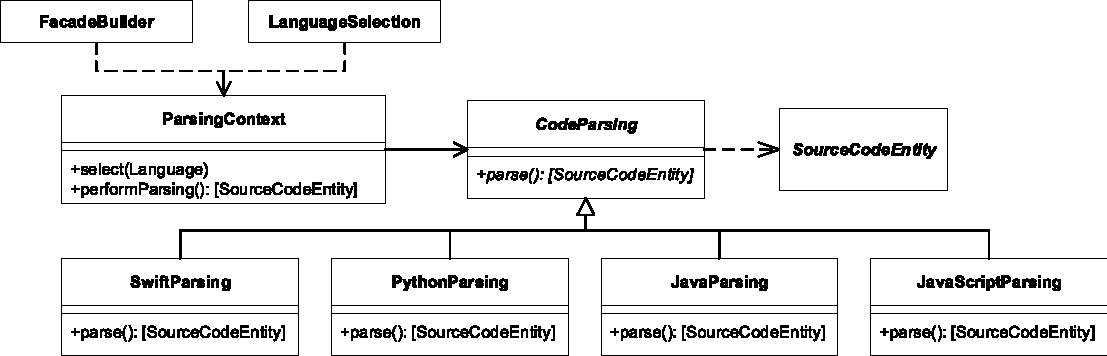
\includegraphics[width=150mm]{images/cd_code_import.pdf}
		\caption{Class diagram of code importer subsystem}
		\label{fig:cdCodeImport}
	}
\end{figure}

Adapting a previous facade to recent changes of a Web API requires importing its source code. Therefore, the \texttt{SourceCode} \texttt{Importer} subsystem must be able to parse source code of multiple programming languages. The decision which programming language needs to be parsed is made during runtime by the user. Since the requirements are the same as for importing different types of \acp{IDL}, the strategy design pattern is also used here. The selection of the programming language to parse is done by the \texttt{Language\-Selection} component while the \texttt{Facade\-Builder} requests the parsed \texttt{Source\-Code\-Entity} objects.

\begin{figure}[!h]
	\centering{
		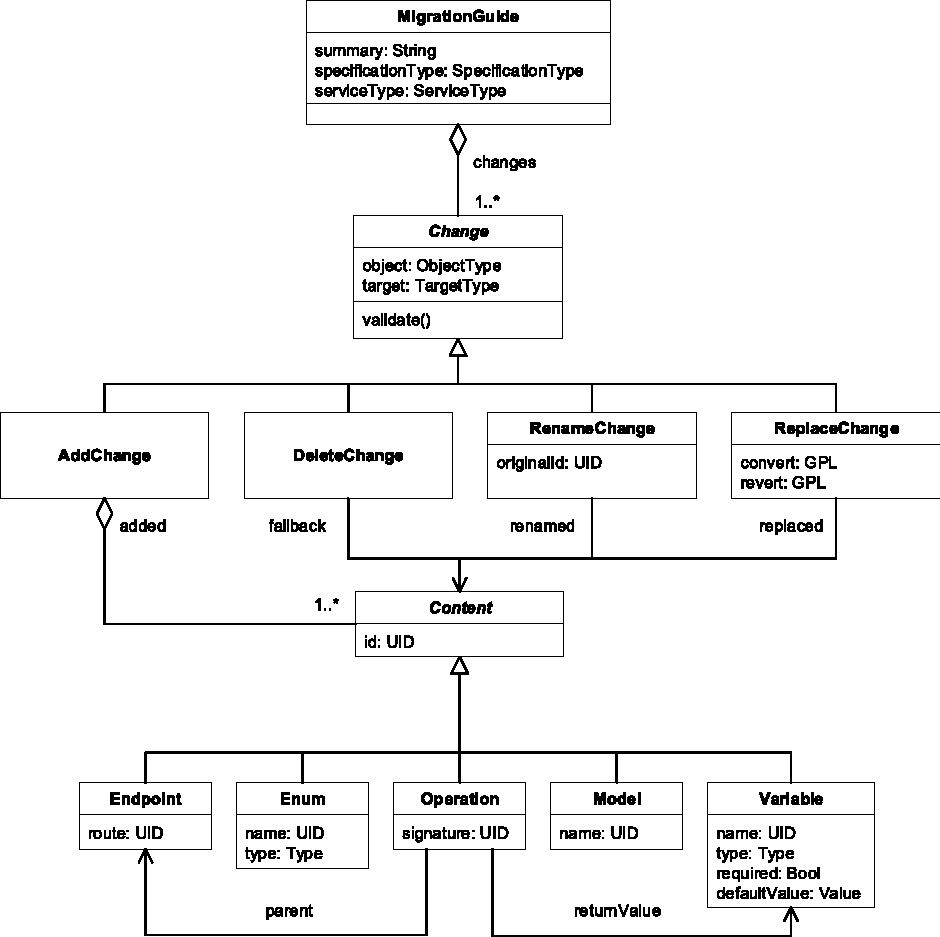
\includegraphics[width=155mm]{images/cd_migguide.pdf}
		\caption{Class diagram of migration guide artifact}
		\label{fig:cdMigrationGuideArtifcat}
	}
\end{figure}

In addition to the decoded representation of the previous facade code, the migration guide needs to be parsed, too. Based on our decision to use \ac{JSON} for defining a migration guide, it can be parsed using a language's core libraries or third-party components. The decoded migration guide structure is shown in Figure \ref{fig:cdMigrationGuideArtifcat}. 

A migration guide contains the type of \ac{IDL} specification in which the Web API is described as well as its service type. Additionally, it specifies all changes that were introduced by the latest version of the Web API. Every change is associated with one of four change types. \texttt{Add\-Changes} denote, that one or more elements of a Web API were added to it. This includes for example adding attributes to a model, parameters to an operation or operations to an endpoint. \texttt{Delete\-Changes} indicate that an element was removed from the Web API. For migratable deletions such as removing an attribute of a model, a fallback value can be specified which is used instead of the removed value. \texttt{Rename\-Changes} are used to automate refactorings. Since the functionality of a renamed element remains unchanged, only the previous and new identifications have to be specified here. 

Elements that were renamed and whose functionality also changed are specified with \texttt{Replace\-Changes}. They are the most complex type of change as they need to contain not only the replacement element, but additionally instructions on how to revert them to their previous version and convert their previous to their current version. Code stated in a \texttt{Replace\-Change} needs to be converted into statements of the programming language specified by the user. Instead of introducing another \ac{DSL} or extending the migration guide \ac{DSL}, we decided to use a \ac{GPL} that is common to web developers. We chose JavaScript for that purpose, as it is one of the most used programming language by web developers and it complements \ac{JSON} well. Furthermore, JavaScript code can be directly executed by an interpreter without previously compiling it. Various programming languages support interpreting JavaScript code. For example, Microsoft provides Windows Script Engines\footnote{https://docs.microsoft.com/en-us/previous-versions/windows/internet-explorer/ie-developer/windows-scripting/windows-script-engines} for C\# and Apple released the framework JavaScriptCore\footnote{https://developer.apple.com/documentation/javascriptcore} for Swift and Objective-C in order to parse and interpret JavaScript at runtime .

Each type of change is applied to one object of the Web API and targets one property of it. For example, adding a parameter to an operation results in an \texttt{Add\-Change} for a \texttt{Operation} object type with a \texttt{Parameter} target type while renaming a model results in a \texttt{Rename\-Change} for a \texttt{Model} object type with a \texttt{Signature} target type. All changes reference \texttt{Content}, i.e. the unique identification of an element of the Web API including additional information that supports the migration process. Invalid changes are indicated by an incorrect combination of their internal information. They are identified by their validation method which reports any errors to the user.

\begin{figure}[!h]
	\centering{
		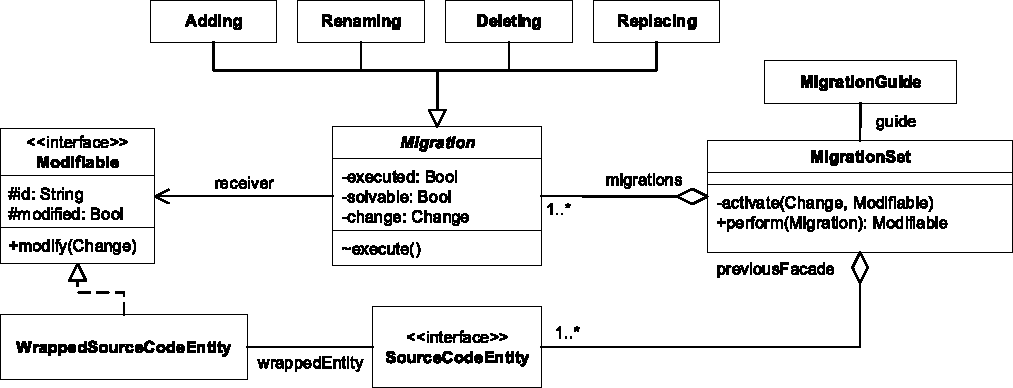
\includegraphics[width=150mm]{images/cd_migration.pdf}
		\caption{Class diagram of migration manager subsystem}
		\label{fig:cdMigrationManager}
	}
\end{figure}

For performing the migration steps, the \texttt{Migration} \texttt{Manager} subsystem incorporates the imported migration guide and decoded previous facade. Analogous to the types of changes, corresponding types of migration are defined. \texttt{Migrations} contain the change that must be migrated as well as information that indicates whether they are solvable and have been executed. Furthermore, they reference a \texttt{Modifiable} object on which the migration is performed. The \texttt{Modifiable} interface is implemented by a wrapper component that acts as an adapter for modifying a \texttt{SourceCodeEntity} of the previous facade. By executing a \texttt{Migration}, the \texttt{modify} method of a \texttt{Modifiable} is triggered which adapts the \texttt{SourceCodeEntity} according to the type of migration. The \texttt{mo\-di\-fied} property of a \texttt{Modifiable} denotes that this object has already been migrated. All migrations as well as the previous facade are composed in the \texttt{MigrationSet}. By analyzing the changes stated in the migration guide and their target entities, it creates the corresponding migrations by invoking the \texttt{ac\-ti\-vate} method. Unsupported or incorrect combinations result in an unsolvable migration. In addition, the user can select a migration strategy to control the migration under certain conditions. The selected migration strategy thereby alters the adaption of source code entities or prevents migrating certain types of changes. Breaking changes that are not migrated automatically must be manually adapted by client developers to fix their application. The \texttt{MigrationSet} is the public interface of the subsystem by providing the \texttt{perform} method to perform a migration and return the adapted facade element.

\begin{figure}[!h]
	\centering{
		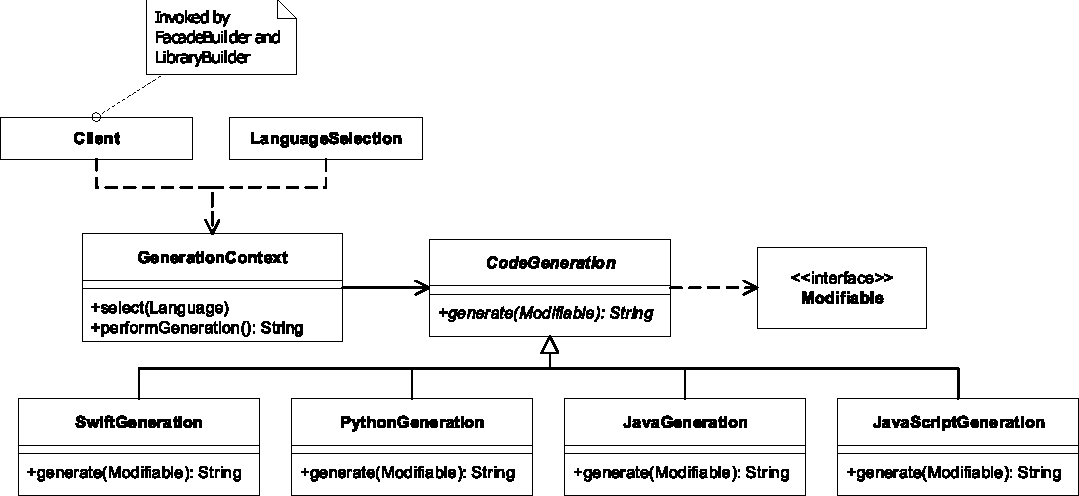
\includegraphics[width=155mm]{images/cd_generation.pdf}
		\caption{Class diagram of code generator subsystem}
		\label{fig:cdGenerator}
	}
\end{figure}

Generating source code from decoded entities for various programming languages requires the \texttt{Code} \texttt{Generator} subsystem to use the strategy pattern. Thereby, it can select the correct syntax elements during runtime. In contrast to the \texttt{Source\-Code} \texttt{Importer} subsystem, it takes \texttt{Modifiable} objects, i.e. wrapped \texttt{Source\-Code\-Entity} objects, as input and generates a string of compilable source code in the programming language the user specified. Its service is used by the subsystems concerned with generating the library code for an IDL and generating the migrated facade code.

\begin{figure}[!h]
	\centering{
		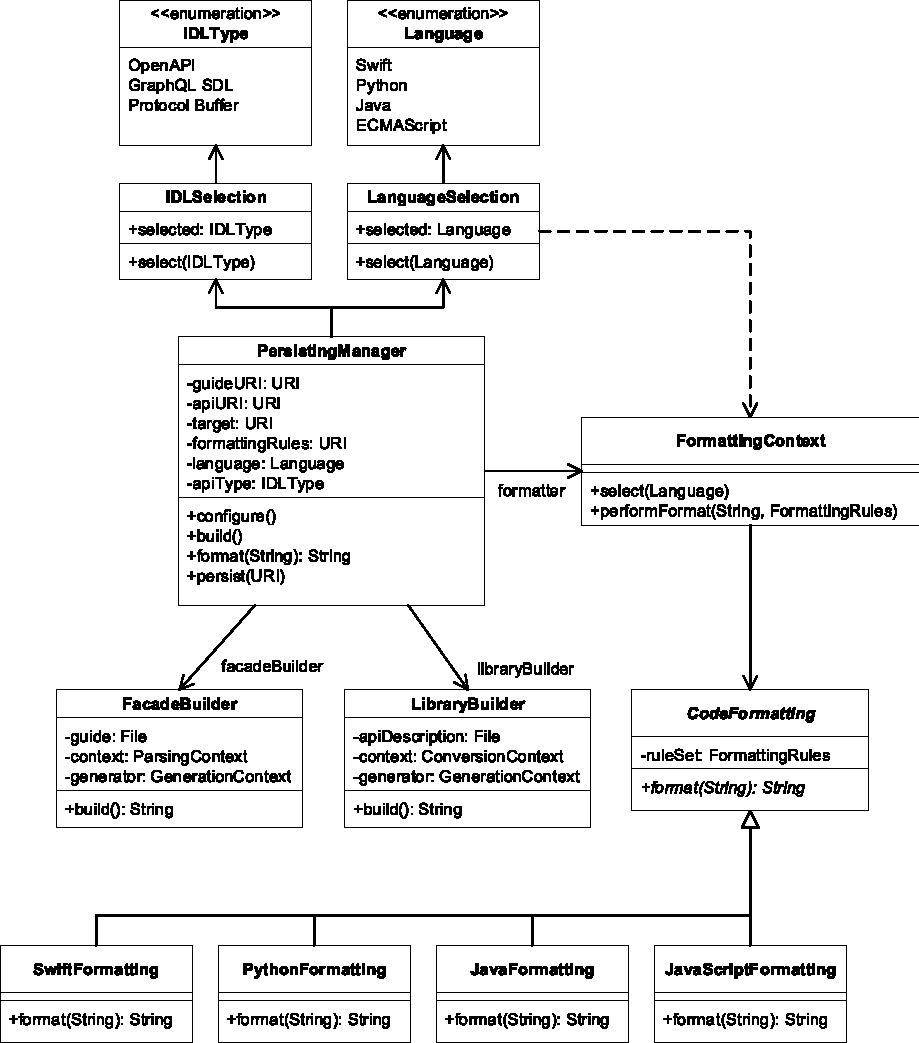
\includegraphics[width=155mm]{images/cd_persisting.pdf}
		\caption{Class diagram of persisting manager subsystem}
		\label{fig:cdPersisting}
	}
\end{figure}

The process is orchestrated by the \texttt{Persisting} \texttt{Manager} subsystem. It takes the user input and selects the desired type of \ac{IDL} and programming language. The selected IDL type results in the initialization of the corresponding concrete strategy of the \texttt{IDL Importer} subsystem. The user's choice of programming language determines the concrete strategy of the \texttt{SourceCode Importer}, \texttt{Code Generation} and \texttt{Code Formatting} subsystems. Additionally, the \texttt{Persisting} \texttt{Manager} contains all configuration options of the user that are necessary to retrieve the Web API's \ac{IDL} and migration guide. Furthermore, it contains the ruleset specifying the formatting style of the source code. After configuring the system according to the user's input, the \texttt{build} method starts the importing, adapting and generating process. Therefore, the \texttt{LibraryBuilder} and \texttt{FacadeBuilder} objects are instantiated and their \texttt{build} method is executed. Both objects hold references to their subsystems that are responsible for generating library code from an imported \ac{IDL} and generating source code of an adapted facade, respectively. Once it receives the generated source code strings, the \texttt{PersistingManager} formats the code using a \texttt{Code\-For\-mat\-ting} component instantiated according to the currently selected programming language. As this is done at runtime, the strategy pattern is also applied here. Formatting source code is available by using third-party components for many programming languages, e.g. SwiftFormat\footnote{https://github.com/apple/swift-format} for Swift and Prettier\footnote{https://prettier.io/} for JavaScript und Java. The formatted source code is then persisted by invoking the \texttt{persist} method. Although the internal structure of the emitted library is defined by our system, the user is able to specify its identifier and its target location.